\chapter{Plasticité classique} \label{chap:Ch10}
\section{Lois de comportement} \label{sec:Ch10-1}
\subsection{Le comportenent plastique} \label{ssec:Ch10-1.1}
Pour les métaux, comme on l'a vu au paragraphe~\ref{ssec:Ch04-2.1}, le comportement est élastique jusqu'à un certain seuil.
Au delà de ce seuil de limite d'élasticité ou de plasticité, le comportement devient plastique, ce qui se traduit en particulier par une non linéarité de la courbe de traction et par une irréversibilité.
\begin{multicols}{2}
    \centering
    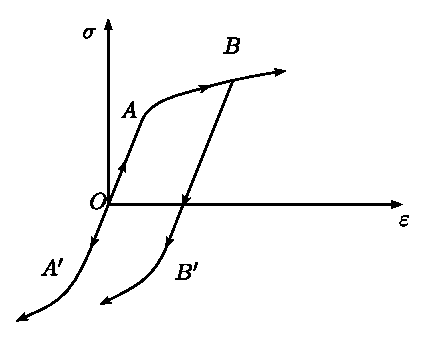
\includegraphics{../images/T1_Ch10-01.eps}
    \columnbreak
    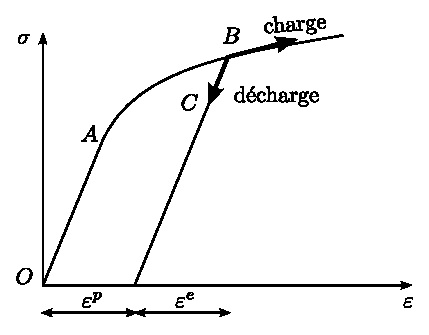
\includegraphics{../images/T1_Ch10-02.eps}
\end{multicols}

Au départ, le matériau se comporte comme un matériau élastique, tant que l'on ne sort pas du domaine élastique initial 
\begin{equation}
    \sigma_{A'} < \sigma < \sigma_A \quad \sigma = E \varepsilon
    \label{eq:Ch10-001}
\end{equation}
avec en général $\sigma_{A'} = - \sigma_A$.
Si l'on charge au delà du seuil, alors apparaissent les déformations plastiques.
Si, arrivé au point $B$, on relâche la contrainte, alors on redescend le long de la droite $BB'$, et le comportement redevient élastique, avec une déformation résiduelle $\varepsilon^p$, et tant que l'on reste dans le nouveau domaine élastique, on a 
\begin{equation}
    \sigma_{B'} < \sigma <\sigma_B \quad \sigma=E \varepsilon^e \quad \varepsilon = \varepsilon^e + \varepsilon^p
    \label{eq:Ch10-002}
\end{equation}
avec en général $\sigma_{B'}\neq - \sigma_{B}$, et même $|\sigma_{B'}|<|\sigma_{A'}|$ (effet Bauschinger). 

Ainsi, on peut à chaque instant décomposer la déformation $\varepsilon$ en une partie élastique $\varepsilon^e$ et une partie plastique ou résiduelle $\varepsilon^p$.
Dans le domaine élastique, la déformation plastique reste constante 
\begin{equation}
    \sigma_{B'} < \sigma <\sigma_B \quad \ud \varepsilon^p = 0
    \label{eq:Ch10-003}
\end{equation}
tandis que si l'on est sur le seuil, $\sigma = \sigma_B$ par exemple, alors on peut avoir un processus de charge avec déformation plastique ou un processus de décharge (retour dans la zone élastique) sans déformation plastique 
\begin{equation}
    \sigma = \sigma_B 
    \begin{cases}
        \ud \alpha \geq 0, \quad \ud \varepsilon^p \geq 0, \quad \ud \sigma_B = K \ud \varepsilon^p \\
        \ud \alpha < 0, \quad \ud \varepsilon^p = 0, \quad \ud \sigma_B = 0
    \end{cases}
    \label{eq:Ch10-004}
\end{equation}
la constante $K$ étant un «~module d'écrouissage~».

On peut simplifier ce comportement élasto-plastique avec écrouissage par un 	comportement idéalisé.
Le modèle le plus simple est celui de la plasticité parfaite, c'est-à-dire sans écrouissage.
Le domaine élastique reste alors fixe
\begin{multicols}{2}
    \centering
    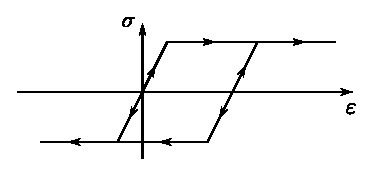
\includegraphics{../images/T1_Ch10-03.eps}
    \columnbreak
    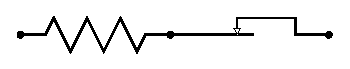
\includegraphics{../images/T1_Ch10-04.eps}
\end{multicols}
C'est le modèle rhéologique décrit au paragraphe~\ref{ssec:Ch04-2.2}.
D'après~\eqref{eq:Ch04-039} et \eqref{eq:Ch04-040}, la loi de comportement de ce modèle peut s'écrire sous la forme 
\begin{equation}
    \sigma = E \varepsilon^e \quad, \quad |\sigma| \leq \sigma_o \quad, \quad \varepsilon = \varepsilon^o + \varepsilon^p 
    \label{eq:Ch10-005}
\end{equation}
\begin{equation}
    \left\{
    \begin{aligned}
        &\dot{\varepsilon}^p = 0  \text{ si } |\sigma| < \sigma_0 \text{ ou } |\sigma| = \sigma_0, \ |\sigma|' < 0 \\
        &\left.
        \begin{aligned}
            \dot{\varepsilon}^p \geq 0 & \text{ si } \sigma = \sigma_0, \dot{\sigma} = 0 \\
            \dot{\varepsilon}^p \leq 0 & \text{ si } \sigma = - \sigma_0, \dot{\sigma} = 0
        \end{aligned}
        \right\} \text{ charge}
    \end{aligned}
    \right.
    \label{eq:Ch10-006}
\end{equation}
Par analogie avec ce que nous avons fait au paragraphe~\ref{ssec:Ch04-1.2} pour les lois de frottement \eqref{eq:Ch04-014} ou pour les conditions de contact unilatéral \eqref{eq:Ch04-013}, nous pouvons réécrire \eqref{eq:Ch10-006} sous une forme plus synthétique 
\begin{equation}
    \dot{\varepsilon}^p = \lambda \text{sign} (\sigma)
    \label{eq:Ch10-007}
\end{equation}
\begin{equation}
    \left\{
    \begin{aligned}
        \text{si} |\sigma| < \sigma_0, & \lambda = 0 \\
        \text{si} |\sigma| = \sigma_0, & \lambda \geq 0, \ |\sigma|' \leq 0, \ \lambda \dot{\sigma} = 0
    \end{aligned}
    \right.
    \label{eq:Ch10-008}
\end{equation}

On utilise aussi parfois, notamment pour des problèmes qui supposent de grandes déformations plastiques (mise en forme des métaux), l'approximation rigide--plastique, qui revient à négliger les déformations élastiques. 
\begin{multicols}{2}
    \centering
    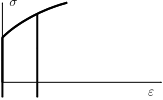
\includegraphics{../image/T1_Ch10-05}
    avec écrouissage
    \columnbreak
    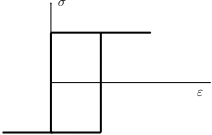
\includegraphics{../image/T1_Ch10-06}
    parfaitement plastique
\end{multicols}

\subsection{Plasticité parfaite}
\endinput
Nous nous limiterons désormais à la plasticité parfaite, qui con­
duit à la théorie classique de la plasticité. Cette théorie peut en effet 
être poussée assez loin, et permet d'obtenir de nombreux résultats. 
La définition du seuil de plasticité dans une théorie tridimension­nelle a fait l'objet du § V.3 . De manière générale, le domaine élastique est défini par 
(9) 

où i est la fonction seuil ou fonction de fluage. En plasticité parfaite, le domaine élastique ne change pas, et cette fonction est définie une fois pour toutes. Dans le cas isotrope, on a discuté au § V.3.1 la forme que pre­
nait ce critère pour les métaux 
(10) = 0
i(Â':~ ) i(J~, J 3 ) ~ 
et les deux cri tères les plus utilisés sont le critère de von Mises 
(j,t
Â
(1 1) .h . . A .. , e. 
'1 ...~
2 2> 
et le critère de Tresca (§ V. 3.2) 
( 12) (cr;, -<Tl ) $ (fe ( (f, ~ <rJ, ~ (J3 ) 
Pour les sols, la pression hydrostatique intervient essentielle­ment dans le critère, et on obtient en général de bons résultats en prenant le critère de Coulomb 
[C'i"" " COOIO-: 
(13) 1 T~ 1 < .c. 

où ..e. est "la cohésion" et if 111' angle de frottement interne". En particu­lier, pour un sol sans cohésion, ~= 0 (cas des matériaux granulaires com­
me le sable), le critère de Coulomb exprime simplement une loi de frotte­ment coulombien sur chaque facette. 

TI:: C'est La critère du type (V.62Y, 
courbE: 
la courbe intrinsèque étant une 
intrinsèque 
droite. 
T" 
Comme dans le cas unidimensionnel, nous décomposons la déformation 
en une partie élastique et une partie plastique 
-1 se ­

(14 ) 

et la contrainte est donnée par une loi élastique en fonction desdéforma­tions élastiques 
(15 ) 

et il reste à compléter la théorie par une loi d'écoulement plastique don­nant l'évolution de la déformation plastique au cours du temps. Il convient donc de g~néraliser la loi \eqref{eq:Ch10-007},\eqref{eq:Ch10-008} du cas unidimensionnel. Auparavant, re­prenons, dans le cas de l'élasta-plasticité, le bilan theITlodynamique expn­mé par (1.60). Compte-tenu de \eqref{eq:Ch10-014} et \eqref{eq:Ch10-015}, nous pouvons écrire 
. e "'\'­
û' :D .. ~ G:. E ~ (J.. E. .. ... V-S· 
.c~ .c~ ...~ .v~ .<.~ .<.~ .<.~ J,.;j 
(16) 


o '-~ . e cl.:W 

~
(J. E. . .,{;,,\\. C· = 
~ô .ca A'<'~k~ A~ dt 
où 'Ur est l'énergie de déforrnat·ion élastique . \eqref{eq:Ch10-017} 
ce qUl permet d'identifier \eqref{eq:Ch10-016} il (l.59) avec 
\eqref{eq:Ch10-018} 

La puissance l'élastique" se transforme en énergie interne élastique, tandis que la puissance "plastique" est dissipée. Le second principe de la thermo­dynamique donne alors l'inégalité 
\eqref{eq:Ch10-018} 
restriction thermodynamique sur la loi d'écoulement plastique. 


1.3 POTENTIEL PLASTIQUE 
seuil 

charge
décharg Domaine 
élastique 
IJ 

'J 
Comme dans le cas unidimensionnel, la déformation plastique reste constante Sl l'on est en évolution élastique, c'est-à-dire si l'on est dans le domai­ne élastique ( '1;<0) ou sur le seuil ~=O si l'on a un processus de dé­charge ( {<O ) 
si i <0 domaine élastique
't
(19) 	E.. : 0 .(.~ t81 {= 0 {<a décharge 
La déformation plastique ne varIe donc que sur le seuil et dans un processus 
de charge (-t=0, t=0). La loi d'évolution est alors habituellement défi­
nie par 
Principe du travail maximal. Dans un état de contraintes ~l~ , le taux de 
déformation plastique vérifie l'inégalité 
.,. 
'"\'­
(20) 	( <r:Ci-Cf.. ) ê .. >--0 
...~
'"* 
.. 	.. 
pour tout (J"•• acceptable, ~ 0
<t 	i ( <r.i.~ ) 
En particulier, il s'ensuit que la restriction thermodynamique \eqref{eq:Ch10-018} 
.. 
est automatiquement vérifiée (il suffit de prendre (J"... ~ =' 0 dans (20», 
Géométriquernent,en se.plaçant dans l'espace vectoriel des contrain­
tes (de dimension 6), l'inégalité \eqref{eq:Ch10-020} se traduit par l'inégalité 
(21) 

~ 0 
où [ est le point représentatif de l'état de contraintes, z:~ un point quel­conque du domaine élastique, et ­
clEf-le vecteur représentatif de l' incré­ment de déformation plastique. 
Si l'on se place en un point du seuil où le plan tangent est conti­nu, alors, en faisant varier L~, on constate que l'inégalité \eqref{eq:Ch10-021} sera vé­rifiée pour tout r." SSi le vecteur incrément de déformation plastique est 

cr· .
'1 
dirigé selon la normale extérieure à la surface seuil en L 
'f­
(22) 
E.. Â 	~ ? ~ 0
'" 
""i d(f:..~ 
La fone tian seuil est un "potentiel plastique". On tire également de \eqref{eq:Ch10-020} la propriété de convexité du domaine élastique 
En effet, SI ce domaine n'est 
pas convexe, alors on constate aisément qu'il est impossible 
.,...... de trouver un vecteur clEt vé­
rifiant \eqref{eq:Ch10-021} pour tout L* 
Ainsi, on tire du principe du travail maximal les propriétés de convexité 
(du domaine élastique) et de normalité (de à la frontière seuil). 
Par analogie avec ce que nous avons fait au § IV.I.2 pour la con­
dition de frottement, nous pouvons réécrire la loi d'écoulement plastique 
sous la forme 
( 
't
1: .. "-a Sl i(<r:..~) < 0 
'i

(23) 
si

€.'1' .. = 'À of l (<f';'a) ~ 0 
"! 
ôa:
"t 
~ ~ 0 0 = 0

1~ Â t 
et la distinction entre processus de charge et de décharge s'effectue au­tomatiquement par le jeu des deux inégalités et de l'inégalité sur? et t Cela peut sembler bien compliqué, c'est néanmoins la "bonne formulation ma­thématique" qui permet de démontrer de nombreux résultats. 
En particulier, si le critère ne dépend pas de la pression hydro­statique forme \eqref{eq:Ch10-010} alors il résulte de \eqref{eq:Ch10-023} que 
(24) = o 
Les déformations plastiques se font à volume constant (incompressibilité plastique) . 
Si  la  surface seuil  ;,::-f.3-~=-:::::  '-"":1  point anguleux  
le cas  du critère de  Tresca  - alors  le  principe du  trava~l maximal  montre  
......  
que  le  vecteur  clEt  est  dans  le  cône  des normales  
Cône  des  normales  

_--Ltf=~ 

Domaine élastique 

Le principe du travail maximal est une hypothèse qUl sera ou non vérifiée selon les matériaux. Elle est vérifiée en première approximation pour les métaux; elle n'est pas vérifiée par contre pour les sols. Ce prin­clpe permet d'engendrer une classe de modèles! les matériaux standard, qui permettent de traiter de nombreux problèmes. Les conclusions obtenues à 
partir de ce type de modèle seront plus ou mo1ns valables selon les problè­
meSa 
Dans le cas du critère de von Mises (II), on obtient 
''\'
(25) 	é '. 
-'-t 


et, par combinaison avec \eqref{eq:Ch10-015}, on a 
(26) 

loi de comportement incrémentale de la plasticité. 
2, EXEMPLES DE PROBLEHES 
======================== 
2 , 1 FLEXION D'UNE POUTRE 
Considérons un arbre êlastoplastique, et soumettons le à un moment 
de flexion 'TQ croissant (voir § VII. 1, l, problèmes 5 et 6). Au départ, la 
solution élastique du § VII.I.3 est valable, et elle le reste tant que 
(27) 

Au delà de "'l,e.' une zone plastique se développe à l'extérieur de la poutre, tandis qu'au milieu subsiste une âme élastique. En supposant que, en chaque 
point, l'état de contraintes reste un état de traction simple (VII.13), nous 
sommes amenés à prendre 
-(Je, 
• ôe (:t~
(28) 
~~ =. 
} 
... cre, 

en supposant la poutre symétrique par rapport à l'axe x
3 Ce èhamp de contrain­
tes vérifie les équations d'é­
quilibre et les CL 	sur la sur­
face latérale. Il vérifie aus-	.x. 
J 
si les CL sur les extrémités 
avec 


b(~) 

et S1 on introduit la fonction ~oc~) donnant la largeur de la poutre en 
-162 ­
fonc t ion de x
2 

où la fonction 'YYl(~) est une fonction qU1 croît de ""1.. donné par \eqref{eq:Ch10-027} à ~donné par 

lorsque '§. décroît de !V..,/J-à 0, c'est-à-dire lorsque la zone plastique s'étend JUS­qu'à occuper tout r 
Il reste à calculer les déplacements. Dans la zone élastique, le calcul du § VII. 1.3 reste valable en remplaçant crrt./-:r par (Je! ~ , et la re­lation (VII.34) devient 
(31 ) 
x. = 
qui, combiné avec \eqref{eq:Ch10-029} , donne la relation entre le moment et la courbure. 
'I1t --~~--,,--­
'fIl.t 


Il reste à étendre cette solution au'domaine plastique, par inté­gration de \eqref{eq:Ch10-023}. Cela pose davantag~ de problèmes, mais il est possible de calculer un champ de déplacements répondant au problème. Ce champ n'est ce­pendant pas unique: en général, on n'a pas unicité du champ de déplacements en plasticité. 
Finalement,. le comportement é1astop1astique d'une poutre en flexion 
est le suivant 
-comportement élastique pour tri\. <: 'YI\.,e au delà de ~: apparition d'une zone plastique, mais les déformations plastiques restent limitées ou "contenues" par le noyau élastique. 
-pour '11\.-mL' le noyau élastique disparaît, et les déformations plas­tiques n'étant plus limitées, il y a ruine de la structure. 
2.2 RESERVOIR SPHERIQUE 
Reprenons en élastoplasticité le problème du réservoir sphérique que nous avons résolu, en élasticité, au § VI.2.2 Si l'on augmente pro­gressivement la pression intérieure 1( , alors la solution élastique reste valable jusqu'à la pression 
\eqref{eq:Ch10-032} 

Au delà, une zone plastique apparaît à l'inrérieur du réservoir. Par raison 
de symétrie, cette zone sera 
limitée par une sphère 1t. .. ~ 

Dans la zone élastique, ~~'I.,.e., l'analyse du § VI.2.2 subsiste, et le ten­seur des contraintes est donné par 


« et ~ étant deux constantes à déterminer. Dans la zone plastique, a.~'!. <~ , d',,?rès la symétrie sphérique du problème, le tenseur des contraintes aura la forme suivante 

où TIC'!.) représente la partie sphérique du tenseur des contraintes, et 't:('t,) son déviateur. Ce tenseur est de révolution autour de la direction radiale, et les contraintes principales sont 

Les équations d'équilibre appliquées à \eqref{eq:Ch10-034} donnent 
\eqref{eq:Ch10-036} 	.2, "t;'C'I.) 1" G 1:('t,) _ ït'(IL) = 0 It. 
équation différentielle reliant les deux fonctions n('!..) et 'CC'\,) . 
D'autre part, dans la zone plastique on doit aVOlr 
= 



en adoptant par exemple le critère de von Mises (comme on l'a vu en VI.2.2 le critère de Tresca donnerait-le même résultat). On en tire donc 
(37) 

(le Ch01X du signe se fait par continuité avec la solution élastique du § VI.2.2). En reportant dans \eqref{eq:Ch10-036} et en intégrant, on obtient 
(38) 

Ainsi, dans le domaine plastique 
/.lC.... ~â'
(39) 0'.. 
~ <Te (~'t, +x) S..~ 0'... Il}
A.t 
(40) 0': 1 ,,(l'J-= ~ (je (~~ +·t) (j'~ = ~ <T~ ( ~IL .. ~ -1! 
où t est une constante d'intégration. Ainsi, le champ de contraintes, défi­
ni par \eqref{eq:Ch10-033} pour ~~Jt.,.Rret par \eqref{eq:Ch10-039} poura..,~,'t., dépend de trois constantes d'intégration ~ ,~ , ~ Ces trois constantes d'intégration s'obtiennent en écrivant la CL en '1. = 1r et la condition de contin~ité de (J'A ' (J'~ et <l', au travers de la surface 't,= ~ . Remarquons ici que la condition de discon-' tinuité (1.22) impose seulement la continuité de <T~ cependant, en plasti­
cité, on doit écrire qu'à la frontière élasto-plastique, l'état élastique est un état limite, ce qui revient à écrire la càntinuité de 0-", et 0"1-. Les 
trois constantes d'intégration étant ainsi déterminées, la CL en '1.= a. donne la valeur de 1" qui correspond à ~ , d'où la fonction t(~) qui croît de f", à ft lorsque ~ croît de Il. jusqu'à ..a-. La valeur limite ft de f s'ob­tient lorsque !. = ir , c'est-à-dire lorsque la zone élastique disparaît. Le champ de contraintes est alors donné par \eqref{eq:Ch10-039}, \eqref{eq:Ch10-040} pour tout 't. . La CL en. '1. = 1r donne alors y et il vient 
(41) 

et en faisant Jt. =Il. on trouve 

(42) 

Comme en 'fl~xion, le réservoir se comporte élastiquement jusqu 1 à 
te . Au delà de +e des déformations plastiques 'apparaissent, mais ces dé­
fonnations restent contenues par la zone élastique jusqu'à ce que t attei­
gne la valeur 1 imite' 1"1. ' qui correspond à la ruine du réservoir. 
3. METHODES VARIATIONNELLES 
=========================== 
3.1 LE PROBLEME EN VITESSES 
En plasticité, il n'y a pas rel'ation biunivoque entre les contrain­tes et les déformations; il est donc tout à fait clair qu'un problème stati­que régulier, tel que nous l'avons formulé au § VI.l.1, est automatiquement mal posé. En effet, l'état de contraintes et de déformations dans un maté­
riau élasto-plastique ne dépend pas seulement de la sollicitation appliquée 
à l'instanr considéré, mais aussi de tout ce qui s'est passé auparavant. Par contre, connaissant l'état actuel de contraintes et de déformations, et con­naissant la variation de sollicitation, on peut espérer trouver la solution. Dans le cadre de l'hypothèse quasi-statique, on est donc amené à se poser un problème incrémentaI (ou problème en vitesses). 

Problème incrémentaI. Connaissaht à l'instant t le champ des contraintes champ des déplacements .l.L... (f):, k) , trouver leurs varia-et .u.l. 0<,,.1;) vérifiant -les équation d'équilibre incrémentaI es 
(43) o
+ t = 
-les c9nditions ~ux limites 
• J. 
(44 ) : 
T·..
<f~~ m~ 1 Sf 
cl.
(45) ..u, . 
..u, ... 15.... = .. 
-la loi de comportement incrémentale 

'1'
avec ~.. donné par la loi d'écoulement plastique.
La 
Si nouS acceptons le principe du travail maximal, c'est encore 
un problème bien posé. 
ThéOrème cl 'unicité. En acceptant le principe du travail maximal, le problème [posé plus haut admet une solution unique en rr·· 
L~ 
Dem. Supposons en effet qu'il existe deux solutions (0-.•. ,i.J..~ ) et (ir.1, ,;"l,).
~à ~ ~~ ~ 
Leur différence 
• 0 • 0 • .t • "'\
." ••
(47) cr .. = 0".. -0".. .u. . .u.. -M.. 
... ... ...
"! "i "'i 
vérifie les équations 
(48 ) , 
(Par contre, elle ne vérifie pas nécessairement la loi de comportement \eqref{eq:Ch10-046} 

• 0 • 0 
qui est non linéaire). En appliq'twnt à <r.. et.u.. le lemme fondamental du "t '" 
§ IX.I. 1 , on obtient alors 
\eqref{eq:Ch10-049} ~ 0 Mais 
. t . tl,· .,
+ <r.. é.. .. -(L . 
.L~ "'i "'~ 
En tout point x, on connait le tenseur des contraintes, on connait donc la 
zone élas tique CL... où f((fL!!) <0 et la zone plas tique n. t où f(<f.;,~) = 0 . 
Dans la zone élastique, les taux de déformations plastiques sont identique­
ment nuls. Dans la zone plastique, on vérifie directement que, d'après le 
principe du travail maximal: 
i\
t-.; • < E. =(). 
(J 
charge décharge 
\eqref{eq:Ch10-050} = 0 ~ 0 
Ainsi, on peut écrire à partir de \eqref{eq:Ch10-049},(5U) 
(51 ) 
~
( 
'.~ .t, . 
= (f é .. .. CT., o
~~ Ni ... ~ Ai
.Qt 
or, est défini positif. On obtient donc 
(52) 

(53) 
cqfd 


Par contre, on ne sait pas démontrer l'unicité des déformations. 
Ces problèmes sont des problèmes mathématiques difficiles et encore mal con­
nus. 
On sait également démontrer des théorèmes variationnels analogues à ceux des § IX J.2 et IX.J.3, qui donnent naissance à des méthodes numéri­ques de solution du problème incrémentai. La résolution d'un problème élas­to-plastique quasi-statique se fait donc pas à pas, par résolution d'une suite de problèmes en vitesses. Mais il est important de remarquer que pour toutes ces questions, la formulation de la loi d'écoulement plastique par le principe du travail maximal joue un rôle essentiel. 
3.2 INTRODUCTION A L'ANALYSE LIMITE 
Nous considérons un problème où le chargement dépend d'un seul paramètre 
S.... = rf ou 

(54)  T.el. ...  =  ? T/o  
Pour les problèmes envisagés  au  §  2,  on  a  '.l.:'hl  pour  la  poutre  en  flexion  
et ').: t  pour le réservoir sphérique.  
Si  l'on fait croître le chargement,  on  obtient  toujours  le même  
' 

comportement. Jusqu'à ~ = ~e la solution élastique convient. Au delà 
apparaît une zone plastique qui progresse au fur et à mesure que ~ aug­mente, et jusqu'à ce que pour'). = ?,t on ait ruine de la structure par dé­
formations plastiques illimitées. 
La charge correspondant à 'il =?,t est appelée "charge limite". C'est la charge maximale supportable et, d'un point de vue pratique, c'est le résultat le plus intéressant et le plus significatif d'un calcul en plas­ticité. On a donc cherché à développer des méthodes permettant de calculer 
directement cette charge limite, sans réso~urion cc~~lète du problème élas­
to-plastique: c'est le domaine de l'analyse limite. 
La théorie s'appuie sur deux théorèmes fondamentaux. 
Défini tion 1. Un champ de contraintes â-.. sera un champ licite pour un 
~~~~~~. ~~ 
chargement (t,T;.,tL) s'il est statiquement admissible et si en tout point 
[ 
il vérifie le critère de plasticité. 
~ 
Définition 2. Un champ de vitesses ~. sera un champ cinématiquement et 
~ 
plastiquement admissible (CCPA) s'il est cinématiquement admissible et si 
0' 
en  chaque point  il existe  un  tenseur  de  contraintes  tel que f... puis­ 
.~  
se  être la déformation plastique associée.  

-168 ­
Dans le cas des métaux par exemple, cette dernière condition re­vient simplement à imposer la condition 
':' 
(55) e .. • o 
..... 
On d~finit alors la fonction de dilsipation 
(56) 

-
N
fonction définie sans ambiguïté, bien qu'il puisse exister plusieurs a:. 
"'a
compatibles avec Pour le critère de von Mises par exemple 

• -i' '-i'
(57) 
E. .' c. .. 
..t ...t 

On peut alors démontrer les deux thêorèmes suivants 
Théorème statique. S'il existe un champ de contraintes licite pour le char­[ gement (J. ,TeL), alors la structure peut supporter ce chargement.
fA. .. 
Théorème cinématique. S'il existe un CCPA tel que 
(58) 

.. (l' TeL 1. cLS )
~s k At 
f 

alors la structure ne peut pas supporter le chargement (p.. ,reL). 
~.. "" 
Le premier théor~me permet de construire des bornes inférieures de la charge limite. En effet, soit â-.~ un CSA pour le chargement (1~ ,T.d.o).
""'6 6"..... .... 
Alors, le champ (').~; ) sera CSA pour le chargement (') ( ,?T"-d.·). En choisissant pour ~ la plus grande valeur conduisant à un champ licite 

ft. 
alors, le thêorème statique permet d'affirmer que ~ est une borne inférieu­re de la charge limite. 
De la même manière, le second théorème permet d'obtenir des bornes supêrieures de la charge limite. Soit en effet 1t~ un CCPA, alors la struc­ture ne pourra pas supporter les chargements vérifiant' (58). La quantité 

est donc une borne supérieure de ~i . On en déduit un encadrement 
(61) 1). , '>-! ~ '). 
qui permet d'approcher relativement simplement la charge limite. On notera 
-169 ­
l'analogie de cette méthode avec celle présentée en élasticit~. 
L'analyse limite est utilis'e 
-en mfcanique des structures, car la charge limite caractérise bien la capacitf de résistance d'une structure -bien mieux en tout cas que la charge élastique-~e -. La tendance actuelle de la règlementation en matiè­re de calcul d'ouvrage consiste à substituer un calcul plastique au calcul élastique traditionnel. 
-pour les problèmes ~mise en forme des métaux (laminage, fiiage, etc.), car elle permet d'évaluer les efforts nécessaires. 
en mécanique des sols, pour calculer la capacité de résistance d'un ouvrage. Il convient alors d'agir avec précaution, car les th'orèmes que nous avons énonc's supposent le principe du travail maximal, principe non vérifié pour les 801s. 
